\subsection{Aufbau}
\begin{minipage}{0.4 \linewidth}
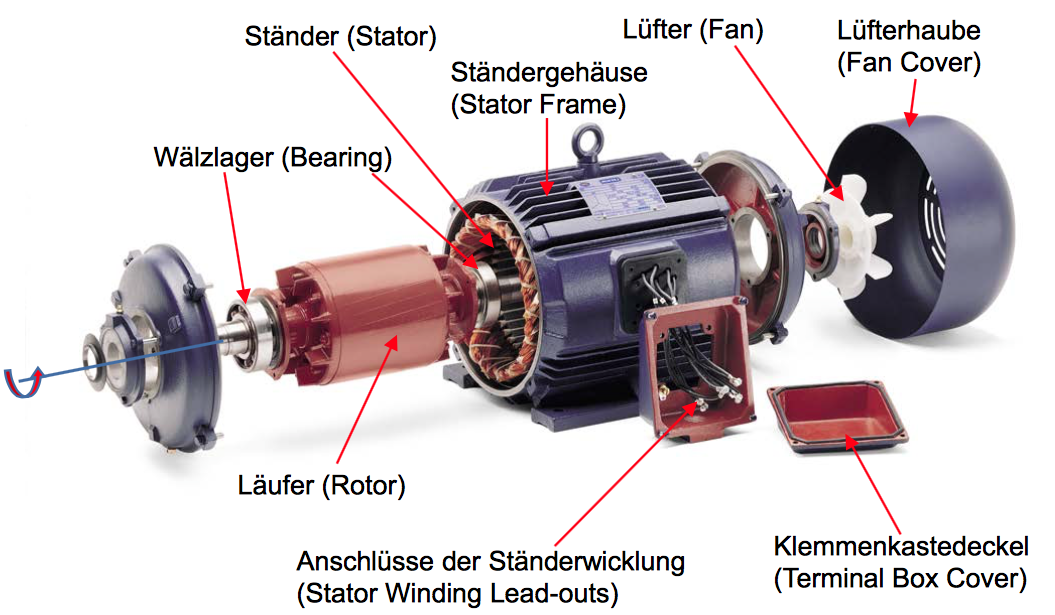
\includegraphics[width = \linewidth]{./Pics/VL1213/Aufbau}
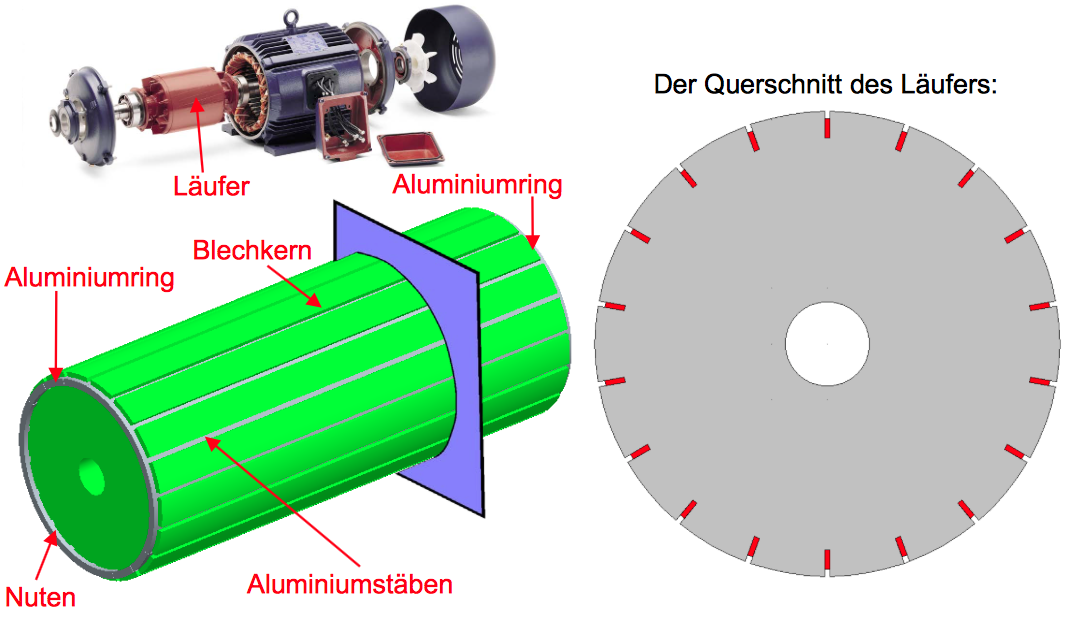
\includegraphics[width = \linewidth]{./Pics/VL1213/Aufbau3}
\end{minipage}
\begin{minipage}{0.4 \linewidth}
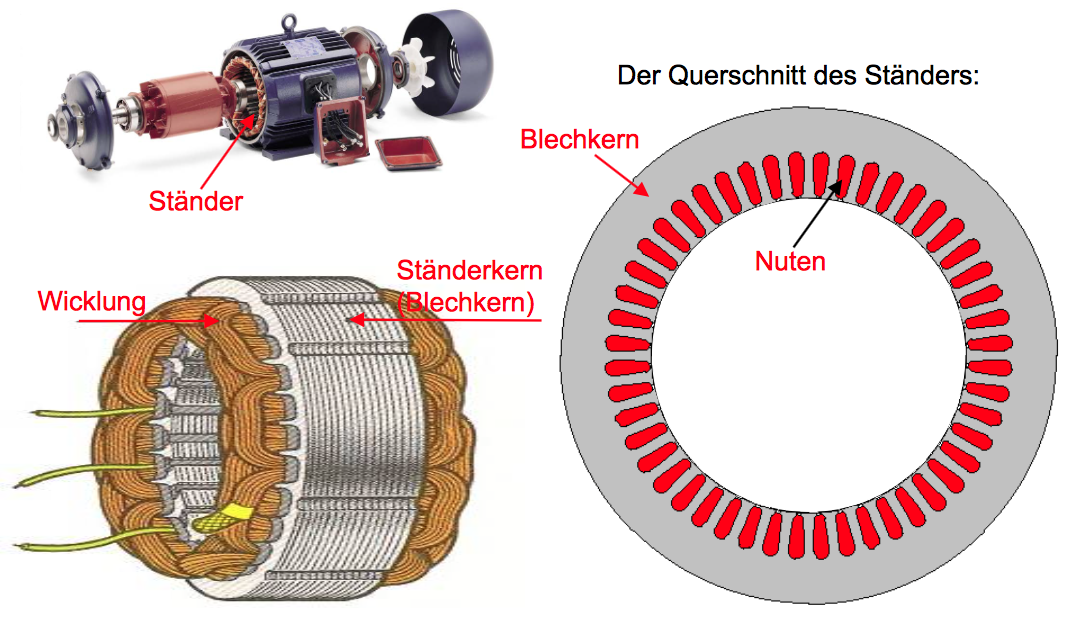
\includegraphics[width = \linewidth]{./Pics/VL1213/Aufbau2}
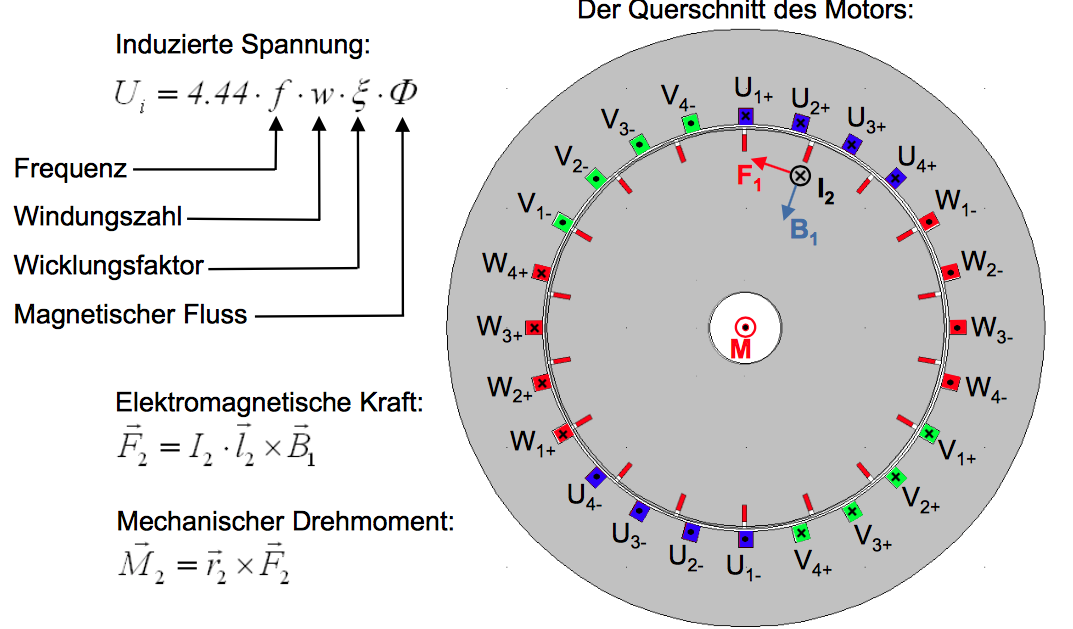
\includegraphics[width = \linewidth]{./Pics/VL1213/Aufbau4}
\end{minipage}

\subsection{Funktion}
\begin{minipage}{0.3 \linewidth}
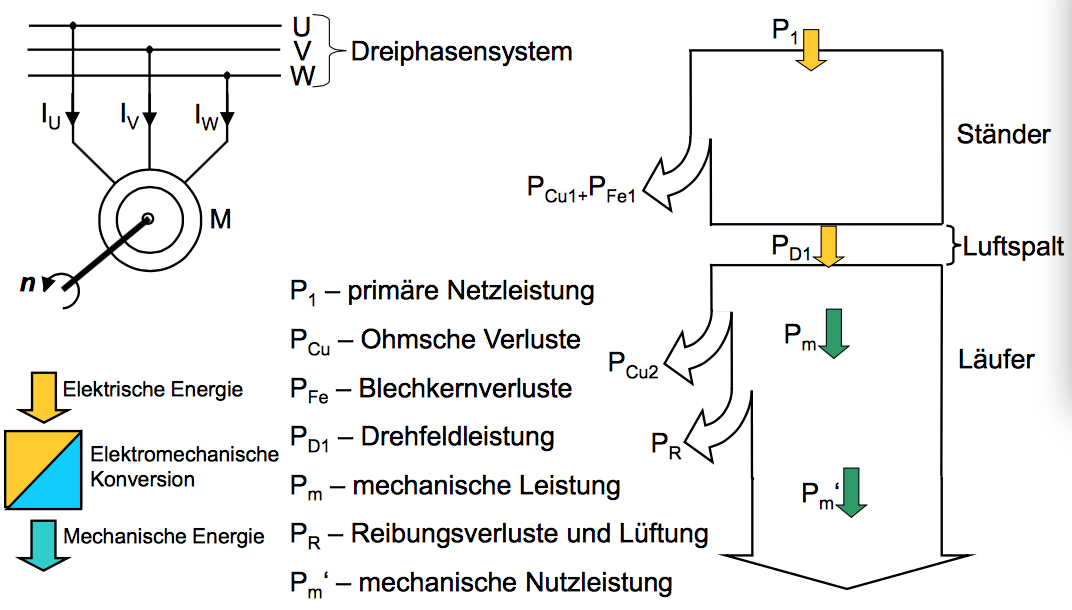
\includegraphics[width = \linewidth]{./Pics/VL1213/Funktion}
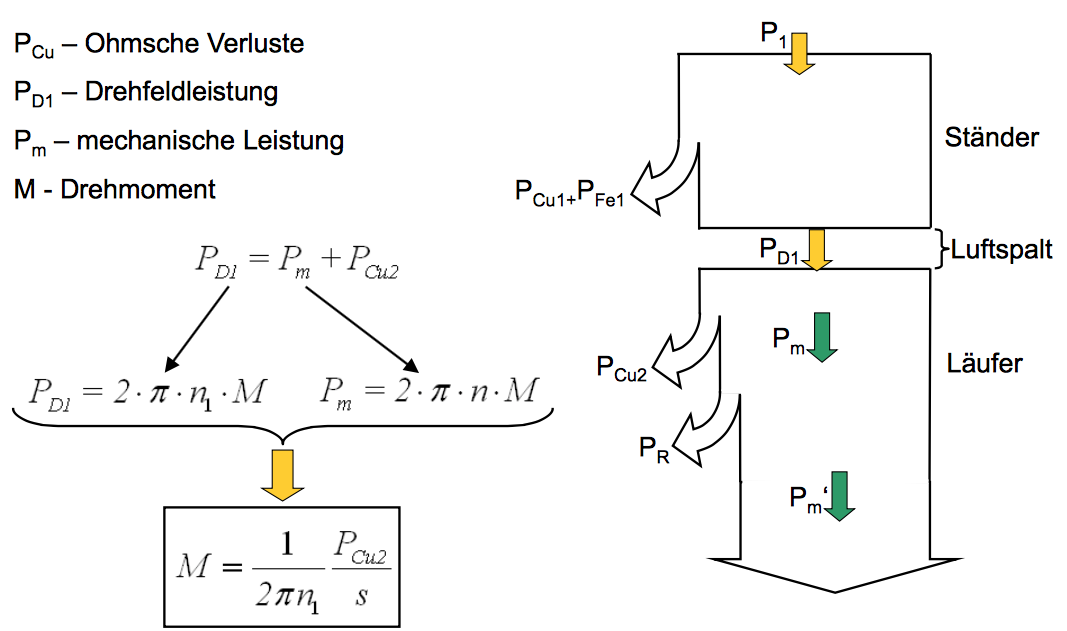
\includegraphics[width = \linewidth]{./Pics/VL1213/Funktion2}
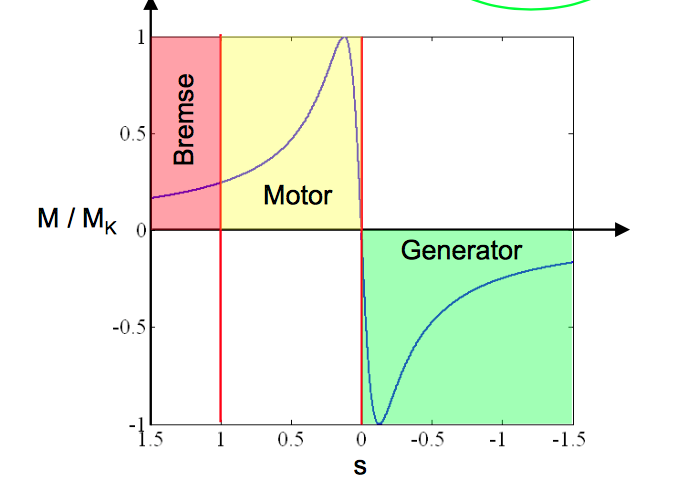
\includegraphics[width = \linewidth]{./Pics/VL1213/Funktion3}
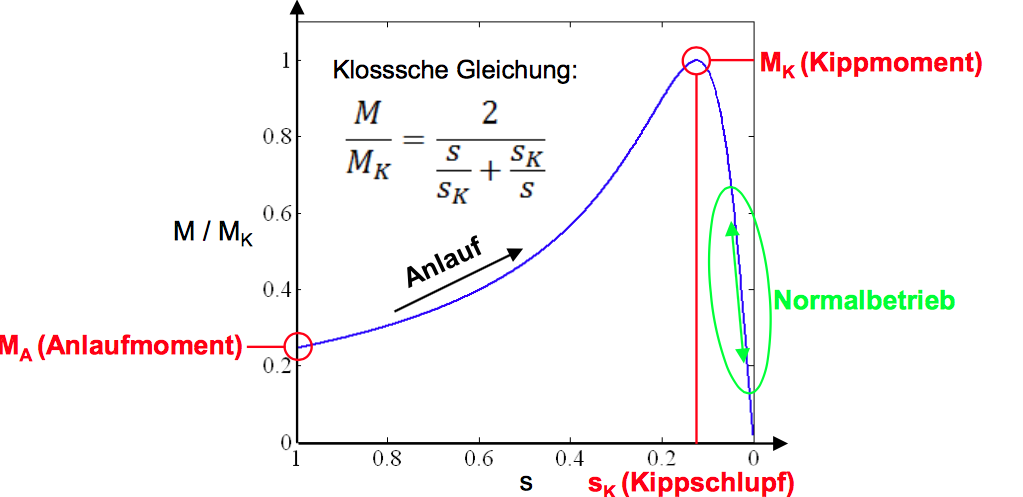
\includegraphics[width = \linewidth]{./Pics/VL1213/Funktion4}
\end{minipage}
\begin{minipage}{0.7 \linewidth}
\begin{itemize}
\item Synchrone Drehzahl (Drehfeld): $n_1 = \frac{f_1}{p}$
\item Drehzahl des Läufers: $n$
\item Realtivdrehzahl: $n_2 = n_1 - n$
\item Schlupf: $s = \frac{n_2}{n_1} = \frac{n_1-n}{n_1} = \frac{f_2}{f_1}$
\item Synchroner Lauf: s = 0
\item Stillstand: s = 1
\item induzierter Strom des Läufers: $I_2 = \frac{U_{i20}}{\sqrt{(\frac{R_2}{s})^2 + X_{2\sigma}^2}}$
\item Stillstand: $s = 1$,$f_2 = f_1$, $I_2 = I_{2max} = \frac{U_{i20}}{\sqrt{R_2^2 + X_{2\sigma}^2}}$
\item Synchroner Lauf: $s = 0$,$f_2 = 0$, $I_2 = I_{2min} = 0$
\item Drehmoment: $M = \frac{1}{2\pi n_1} \frac{P_{cu2}}{s} = \frac{q_2}{2\pi n_1} I_2^2 \frac{R_2}{s} = \frac{q_2}{2 \pi n_1} \frac{U_{i20}^2}{\frac{R_2}{s}^2 + X_{2\sigma}^2} \frac{R_2}{s}$
\item Drehmoment Anlauf: $M = \frac{q_1}{2 \pi n_1} \cdot \frac{U_1^2}{\frac{R'_2}{s}^2 + X'^2_{2\sigma}} \cdot \frac{R'_2}{s}$
\item Schlupf Kippmoment: $s_k = \frac{R'_2}{X'_{2\sigma}}$
\item Kippmoment: $M_K = \frac{q_1}{4\pi n_1} \cdot \frac{U_1^2}{X'_{2\sigma}}$
\item Leerlaufstrom: $\underline{I_0} = \underline{I_{fe}} + \underline{I_\mu}$
\item Klossche Gleichung: $\frac{M}{M_K} = \frac{2}{\frac{s}{s_k} + \frac{s_k}{s}}$
\end{itemize}
\end{minipage}

\subsection{Model der ASM}
\begin{minipage}{0.3 \linewidth}
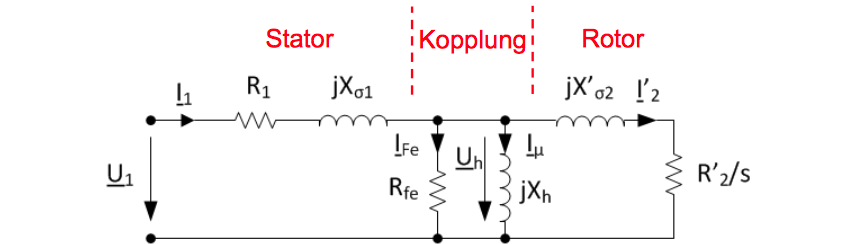
\includegraphics[width = \linewidth]{./Pics/VL1213/ModellASM} \\
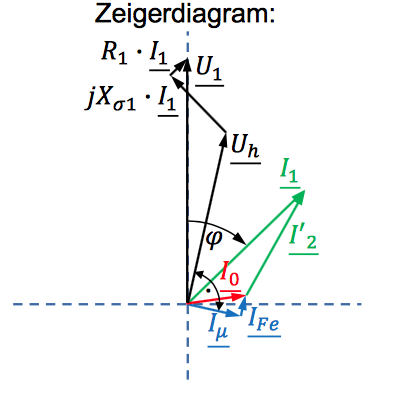
\includegraphics[width = 0.5 \linewidth]{./Pics/VL1213/Zeigerdiagramm}
\end{minipage}
\begin{minipage}{0.3 \linewidth}
\begin{itemize}
\item Grundgleichungen: 
\begin{itemize}
\item $\underline{I_1} = \underline{I_{Fe}} + \underline{I_\mu} + \underline{I_2}$ 
\item $\underline{U_1} = R_1 \cdot \underline{I_1} + jX{\sigma 1} \cdot \underline{I_1} + U_h$
\end{itemize}
Übersetzungsverhältnis:
\begin{itemize}
\item $u = \frac{N_1 \cdot k_{w1}}{N_2 \cdot k_{w2}}$
\item $\underline{I'_2} = \underline{I_2} \cdot u$
\item $R'_2 = R_2 \cdot u^2$  
\end{itemize}
\end{itemize}
\end{minipage}
\begin{minipage}{0.4\linewidth}
\begin{compactitem}
\item N - Windungszahl
\item $k_w$ Wicklungsfaktor
\item $R_1$ Widerstand des Stators
\item $R_2$ Widerstand des Rotors
\item $X_{\sigma 1}$ Streureaktanz des Stators
\item $X_{\sigma 2}$ Streureaktanz des Rotors
\item $R_{fe}$ Eisen-Verluste
\item $X_h$ - Hauptreaktanz
\item $U_h$ - innere Spannung
\item $I_\mu$ - Magnetisierungsstrom
\end{compactitem}
\end{minipage}
\subsubsection{Leerlauf}
\begin{minipage}{0.3 \linewidth}
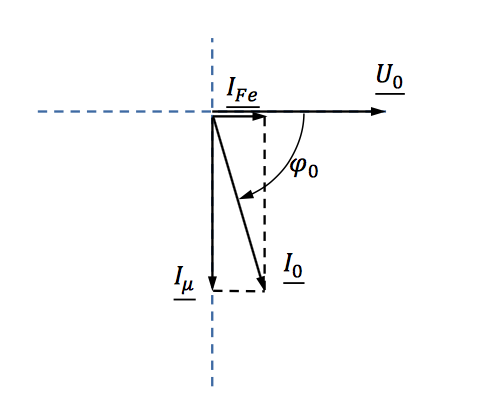
\includegraphics[width = \linewidth]{./Pics/VL1213/ZeigerdiagrammLeer}
\end{minipage}
\begin{minipage}{0.4 \linewidth}
$cos \varphi_0 = \frac{P_0}{U_0 \cdot I_0}$ \\

$R_{Fe} = \frac{U_0}{I_{Fe}} = \frac{U_0}{I_0 \cdot cos\varphi_0}$ \\

$X_h = \frac{U_0}{I_\mu} = \frac{U_0}{I_0 \cdot sin\varphi_0}$\\
\end{minipage}
\begin{minipage}{0.3 \linewidth}
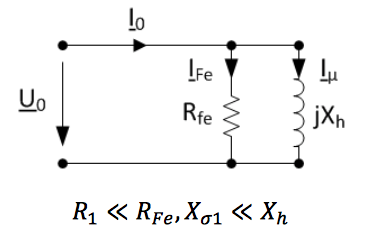
\includegraphics[width = \linewidth]{./Pics/VL1213/Leerlauf}
\end{minipage}

\subsubsection{Kurzschluss}
\begin{minipage}{0.3 \linewidth}
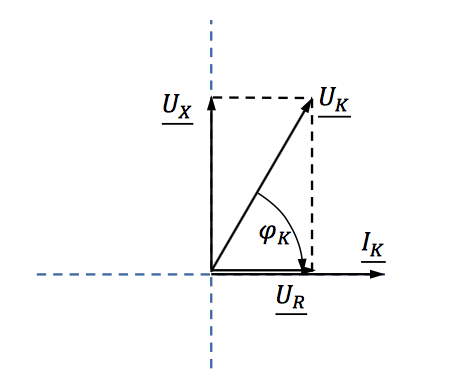
\includegraphics[width = \linewidth]{./Pics/VL1213/ZeigerdiagrammKurz}
\end{minipage}
\begin{minipage}{0.4 \linewidth}
$cos \varphi_K = \frac{P_K}{U_K \cdot I_K}$ \\

$R_{1} + R'_2 = \frac{U_K}{I_K} = \frac{U_K \cdot cos\varphi_K}{I_K}$ \\

$X_{\sigma 1} + X'_{\sigma 2} = \frac{U_X}{I_K} = \frac{U_K \cdot sin\varphi_l}{I_K}$\\
\end{minipage}
\begin{minipage}{0.3 \linewidth}
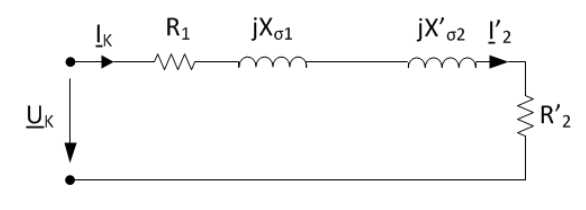
\includegraphics[width = \linewidth]{./Pics/VL1213/Kurzschluss}
\end{minipage}

\begin{minipage}{0.4 \linewidth}
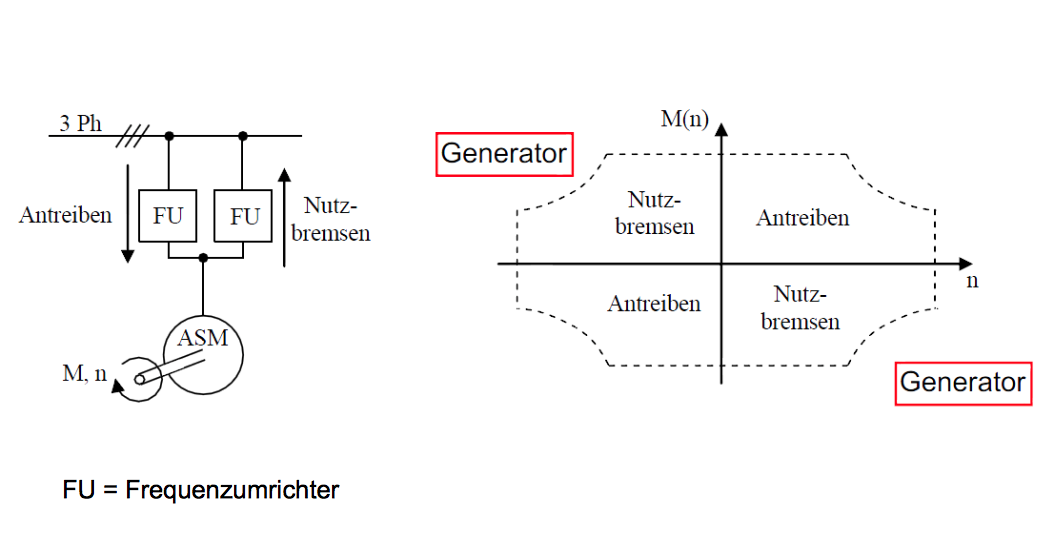
\includegraphics[width = \linewidth]{./Pics/VL1213/Umrichter}
\end{minipage}
\begin{minipage}{0.6 \linewidth}
\subsection{Anwendungsbeispiele}
\begin{itemize}
\item Der Asynchronmotor ist heute der am meisten verwendete Elektromotor
\item Die Konstruktion des Asynchronmotors ist nicht kompliziert.
\item Der Ständer erzeugt das magnetische Drehfeld
\item Das Drehmoment wird durch den Läufer im induzierten Strom erzeugt
\item Der Anlauf des Motors könnte wegen dem Anlaufstrom problematisch sein.
\item Der Asynchronmotor hat einen hohen Wirkungsgrad (80-90\%).
\item Der Läufer ist sehr robust und elektrodynamisch, mechanisch und thermisch stabil.
\item Das Drehmoment des Motors ist bei der Entwicklung einfach zu bestimmen.
\end{itemize}
\end{minipage}